% Week 8 lecture notes: Multimodal Models
% Generative AI (CS 782/882), Old Dominion University, Fall 2026
% Compile with: pdflatex -interaction=nonstopmode week08-notes.tex  (run twice)

% Shared preamble for the Generative AI (CS 782/882, Fall 2026) lecture notes.
% Each weekNN-notes.tex file inlines this block so it compiles on its own.
\documentclass[11pt]{article}
\usepackage[margin=1in]{geometry}
\usepackage[T1]{fontenc}
\usepackage[utf8]{inputenc}
\usepackage{lmodern}
\usepackage{amsmath,amssymb,amsthm,mathtools,bm}
\usepackage{enumitem}
\usepackage{graphicx}
\usepackage{booktabs}
\usepackage{xcolor}
\usepackage{tikz}
\usetikzlibrary{arrows.meta,positioning,calc,shapes}
\usepackage{listings}
\usepackage[colorlinks=true,linkcolor=blue!60!black,urlcolor=blue!60!black,citecolor=blue!60!black]{hyperref}

\newcommand{\E}{\mathbb{E}}
\newcommand{\Var}{\mathrm{Var}}
\newcommand{\KL}{\mathrm{KL}}
\newcommand{\given}{\,\vert\,}
\newcommand{\R}{\mathbb{R}}
\DeclareMathOperator*{\argmax}{arg\,max}
\DeclareMathOperator*{\argmin}{arg\,min}
\newtheorem{theorem}{Theorem}
\newtheorem{lemma}{Lemma}
\newtheorem{definition}{Definition}
\theoremstyle{remark}
\newtheorem*{remark}{Remark}

\lstset{basicstyle=\ttfamily\small,breaklines=true,frame=single,columns=fullflexible}
% ---- end of shared preamble ----

% Week-specific additions.
\usepackage{pdflscape}
\usepackage{array}
\newcommand{\fimg}{f_{\text{img}}}
\newcommand{\ftxt}{f_{\text{txt}}}
\newcommand{\simop}{\mathrm{sim}}
\newcommand{\plain}[1]{\medskip\noindent\textit{Plain English:} #1\medskip}

\title{Week 8 Lecture Notes: Multimodal Models}
\author{Hong Qin, Old Dominion University}
\date{Fall 2026}

\begin{document}
\maketitle

\begin{center}
\textit{Audience:} Graduate students finishing an eight-week course on generative AI.\\
\textit{Goal:} Understand joint embedding spaces, the contrastive (InfoNCE) objective behind CLIP, the systems built on top of CLIP-style embeddings (text-to-image generators, multimodal LLMs, audio and video models), and how to evaluate and responsibly deploy any of the seven model families covered in this course.
\end{center}

\tableofcontents
\bigskip
\hrule
\bigskip

\section*{Acronyms and Notation}
\begin{description}[style=nextline,leftmargin=1.8em,labelsep=0.6em]
  \item[CLIP] Contrastive Language-Image Pretraining (Radford et al., 2021). Two encoders trained with a symmetric contrastive loss on 400 million image-text pairs.
  \item[InfoNCE] The contrastive loss introduced by van den Oord et al.\ (2018); a softmax cross-entropy over one positive pair and many negative pairs.
  \item[ViT] Vision Transformer; an image encoder that treats image patches as tokens.
  \item[LLM / VLM] Large language model / vision-language model (an LLM that also accepts image input).
  \item[$x_i, y_i$] The $i$-th image and its paired caption.
  \item[$\fimg, \ftxt$] Image encoder and text encoder, each mapping into $\R^d$.
  \item[$\simop(x,y)$] Similarity between an image and a caption; dot product of the two embeddings (cosine similarity after L2 normalization).
  \item[$\tau$] Temperature that scales the similarities before the softmax.
  \item[$N$] Batch size (number of image-caption pairs in one training step).
  \item[$z_{\text{text}}, z_{\text{img}}$] CLIP text embedding and CLIP image embedding of the same concept (used by DALL-E 2).
\end{description}

% =====================================================================
\section{Topic 1: Shared Representations Across Modalities}
% =====================================================================

\subsection*{Plain-English summary first}
The single most consequential idea in modern multimodal AI is the \emph{joint embedding space}: train one encoder per modality so that each maps its inputs into the same vector space. Once a $d$-dimensional vector can represent either an image or its caption, you can compare image to image, caption to caption, or image to caption with the same dot-product operation. Retrieval becomes vector search. Classification becomes an $\argmax$ over candidate-class embeddings. Conditional generation becomes ``decode something whose embedding matches this target embedding.'' This Topic sets up the framework; Topic 2 covers the contrastive training procedure that makes it work; Topic 3 surveys the systems built on top.

\subsection{The setup: paired data and two encoders}
Consider a dataset of image-caption pairs
\[
\{(x_i, y_i)\}_{i=1}^{N}, \qquad x_i = \text{an image},\quad y_i = \text{the caption that describes it}.
\]
The standard approach has three pieces:
\begin{itemize}[leftmargin=1.4em]
  \item An \textbf{image encoder} $\fimg : \text{images} \to \R^d$. A vision transformer (ViT) or a ResNet-50 are typical choices.
  \item A \textbf{text encoder} $\ftxt : \text{captions} \to \R^d$. A transformer (Module 6) is the standard choice.
  \item A \textbf{training objective} that pushes matched pairs $(x_i, y_i)$ to nearby vectors and unmatched pairs $(x_i, y_j)$, $j \neq i$, to far-apart vectors. Topic 2 covers this in detail.
\end{itemize}
After training, the two encoders \emph{independently} produce $d$-dimensional vectors in a shared space. The bet is that shared structure (``cat-ness,'' ``sunset-ness,'' and so on) is captured along consistent directions in this space regardless of which encoder produced the vector.

\plain{Nothing about a vector space knows what an image or a sentence is. The only thing that makes $\fimg(x)$ and $\ftxt(y)$ comparable is that they were trained \emph{together} against an objective that rewards agreement on matched pairs. The space is shared because the loss forced it to be.}

\subsection{Cosine similarity and L2 normalization}
Two vectors $u, v \in \R^d$ are compared with the cosine similarity
\begin{equation}
\cos(u, v) \;=\; \frac{u \cdot v}{\|u\|_2 \, \|v\|_2},
\label{eq:cosine}
\end{equation}
which ranges from $-1$ (opposite direction) to $+1$ (same direction), with $0$ meaning orthogonal. The standard practice is to \emph{L2-normalize} every embedding,
\[
\hat{u} = \frac{u}{\|u\|_2}, \qquad \|\hat{u}\|_2 = 1,
\]
so that all embeddings live on the unit sphere and cosine similarity reduces to a plain dot product:
\[
\cos(u,v) = \hat{u} \cdot \hat{v}.
\]

\plain{Normalization throws away the \emph{length} of each embedding and keeps only its \emph{direction}. Length is a nuisance quantity here (a brighter image or a longer caption should not automatically be ``more similar'' to everything), while direction is where the semantic content lives. Once everything is on the sphere, a similarity search is a single matrix-vector product, which is why this scales to billions of items.}

\subsection{Cross-modal retrieval as the canonical use}
Once you have a joint embedding space, the natural first application is \textbf{cross-modal retrieval}: search images by text, or text by images. The procedure has two phases.
\begin{enumerate}[leftmargin=1.6em]
  \item \textbf{Indexing time.} Embed every candidate item in the gallery (for example, all images in a dataset) and store the normalized vectors $\hat{g}_1, \dots, \hat{g}_M$.
  \item \textbf{Query time.} Embed the query $q$ in the \emph{other} modality, compute its similarity to every gallery vector, and return the top-$k$:
  \[
  \text{score}_m = \hat{q} \cdot \hat{g}_m, \qquad
  \text{retrieve } \operatorname{top-}k \text{ of } \{\text{score}_1, \dots, \text{score}_M\}.
  \]
\end{enumerate}
This is how modern visual search engines work: the ``search'' is a nearest-neighbor lookup in embedding space.

\subsection{Aligned versus grounded representations}
Two terms appear in the literature with different meanings:
\begin{itemize}[leftmargin=1.4em]
  \item \textbf{Aligned:} an image and its caption map to nearby vectors. The model knows \emph{which} images and captions correspond, but not necessarily which objects in the image correspond to which words in the caption.
  \item \textbf{Grounded:} the model can localize \emph{which region} of an image corresponds to \emph{which word} in the caption. This is stronger than alignment and requires either bounding-box supervision or attention-based methods.
\end{itemize}
CLIP-style models are aligned but not grounded. Grounded models (GLIP, the captioning side of Flamingo) do extra work. Aligned models are vastly more common because paired image-caption data is far easier to obtain than region-level annotations.

\subsection{Why the recipe generalizes beyond text and image}
The joint-embedding idea applies to any pair of modalities with naturally paired data. The recipe is always the same: two encoders, a contrastive objective, one shared latent space.
\begin{itemize}[leftmargin=1.4em]
  \item \textbf{Audio + text:} train on transcribed speech; the result is Whisper-style audio-text models.
  \item \textbf{Video + text:} train on subtitled or captioned video; the result is VideoCLIP-style models and the conditioning module inside text-to-video generators.
  \item \textbf{Image + image:} train on different views of the same scene; the result is self-supervised vision models such as SimCLR and DINO.
  \item \textbf{Code + natural language:} train on code paired with docstrings or commit messages; the result is code-search systems.
  \item \textbf{Protein sequence + protein structure:} train on paired sequence-structure data; the result is the embedding spaces underlying AlphaFold and ESM.
\end{itemize}

\subsection{Connection to earlier modules}
You have already seen every piece. The image encoder is a CNN or a transformer (Module 6). The text encoder is a transformer (Module 6). The shared latent space generalizes the Module 2 latent-variable setup, except that now \emph{two} encoders feed the same space rather than one encoder per observation. The decoder of choice is usually a diffusion model conditioned on the multimodal embedding (Module 5).

\subsection*{Plain-English payoff}
A joint embedding space turns three seemingly different problems (retrieval, classification, conditional generation) into one problem: compare vectors. Everything downstream in this module, from zero-shot classification to text-to-image generation to ``chat models that can see,'' rests on this one design decision. The remaining question is how to train the two encoders so that the space actually has the property we want; that is Topic 2.

% =====================================================================
\section{Topic 2: Contrastive Learning and Text-Image Alignment}
% =====================================================================

\subsection*{Plain-English summary first}
Training a joint embedding space requires telling the encoders ``this image and this caption belong together; that image and that other caption do not.'' The trick of contrastive learning is that you do not need explicit negative labels: within a batch, every pair other than the matched one is treated as a negative. Combined with massive scale (CLIP trained on 400 million image-text pairs scraped from the web), this produces a joint embedding that supports zero-shot classification. This Topic walks through the contrastive loss, the CLIP architecture, the zero-shot trick, and the modern variants.

\subsection{The similarity matrix}
Take a batch of $N$ image-caption pairs. Embed all $N$ images and all $N$ captions, normalize, and form the $N \times N$ matrix of similarities
\begin{equation}
S_{ij} \;=\; \simop(x_i, y_j) \;=\; \fimg(x_i) \cdot \ftxt(y_j), \qquad i, j = 1, \dots, N,
\label{eq:simmatrix}
\end{equation}
where the dot product equals the cosine similarity of Eq.~\eqref{eq:cosine} because the embeddings are L2-normalized. The training objective is: \emph{make the diagonal entries $S_{ii}$ large and the off-diagonal entries $S_{ij}$, $i \neq j$, small.} The diagonal holds the matched pairs (the image in row $i$ goes with the caption in column $i$); the off-diagonals hold the mismatched (negative) pairs.

\plain{Every batch of $N$ matched pairs gives you $N(N-1)$ \emph{free} negative pairs without any extra labeling. Scale the batch to tens of thousands of examples and each step carries hundreds of millions of training signals. This is what makes contrastive learning data-efficient.}

\begin{figure}[ht]
\centering
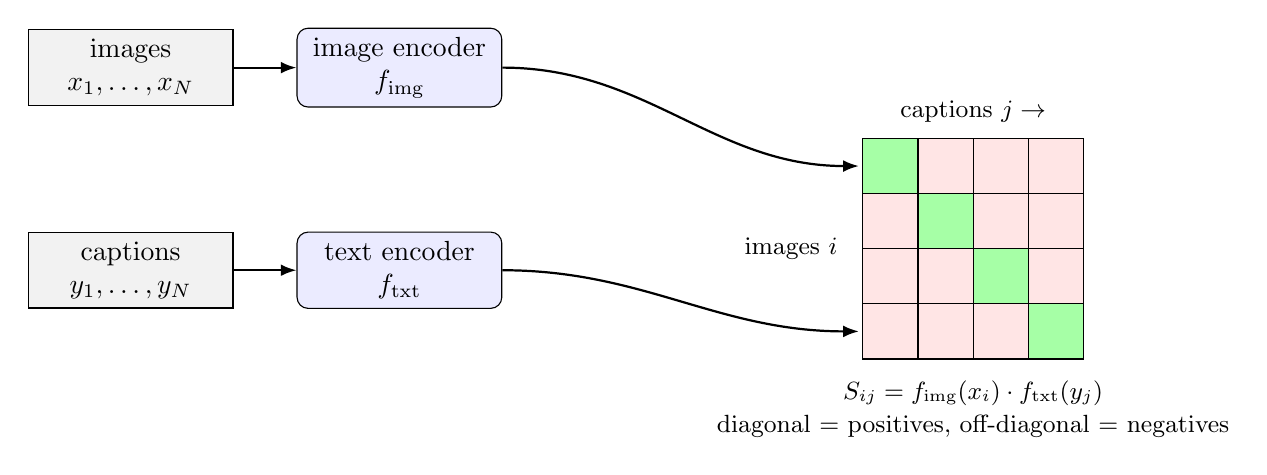
\begin{tikzpicture}[
  enc/.style={draw, rounded corners, minimum width=2.6cm, minimum height=0.9cm, fill=blue!8, align=center},
  inp/.style={draw, minimum width=2.6cm, minimum height=0.8cm, fill=gray!10, align=center},
  arr/.style={-{Latex[length=2mm]}, thick}
]
  % image tower
  \node[inp] (imgs) at (0,0) {images\\ $x_1,\dots,x_N$};
  \node[enc, right=0.8cm of imgs] (fimg) {image encoder\\ $\fimg$};
  % text tower
  \node[inp, below=1.6cm of imgs] (txts) {captions\\ $y_1,\dots,y_N$};
  \node[enc, right=0.8cm of txts] (ftxt) {text encoder\\ $\ftxt$};
  \draw[arr] (imgs) to (fimg);
  \draw[arr] (txts) to (ftxt);
  % similarity matrix (4x4 grid)
  \coordinate (origin) at (9.3,-0.9);
  \foreach \i in {0,1,2,3} {
    \foreach \j in {0,1,2,3} {
      \ifnum\i=\j
        \fill[green!35] ($(origin)+(\j*0.7,-\i*0.7-0.7)$) rectangle ++(0.7,0.7);
      \else
        \fill[red!10] ($(origin)+(\j*0.7,-\i*0.7-0.7)$) rectangle ++(0.7,0.7);
      \fi
      \draw ($(origin)+(\j*0.7,-\i*0.7-0.7)$) rectangle ++(0.7,0.7);
    }
  }
  \node[anchor=south] at ($(origin)+(1.4,0.08)$) {\small captions $j \rightarrow$};
  \node[anchor=east] at ($(origin)+(-0.2,-1.4)$) {\small images $i$};
  \node[anchor=north, align=center] at ($(origin)+(1.4,-2.95)$) {\small $S_{ij} = \fimg(x_i)\cdot\ftxt(y_j)$\\ \small diagonal = positives, off-diagonal = negatives};
  % arrows from encoders into matrix
  \draw[arr] (fimg.east) to[out=0,in=180] ($(origin)+(-0.05,-0.35)$);
  \draw[arr] (ftxt.east) to[out=0,in=180] ($(origin)+(-0.05,-2.45)$);
\end{tikzpicture}
\caption{CLIP's dual-encoder design. Two independent encoders map images and captions into one $d$-dimensional space; the $N\times N$ similarity matrix compares every image with every caption in the batch. Training pushes the diagonal up and the off-diagonal down.}
\label{fig:clip}
\end{figure}

\subsection{The InfoNCE loss}
The standard contrastive loss is symmetric across image-to-text and text-to-image lookups. For image $i$, the loss pushes its own caption $y_i$ to be the most similar caption in the batch:
\begin{equation}
\mathcal{L}_{\text{i2t}} \;=\; -\frac{1}{N}\sum_{i=1}^{N} \log
\frac{\exp\!\big(\simop(x_i, y_i)/\tau\big)}{\sum_{j=1}^{N}\exp\!\big(\simop(x_i, y_j)/\tau\big)},
\label{eq:i2t}
\end{equation}
where $\tau$ is a temperature parameter. In CLIP, $\tau$ is learnable and initialized near $0.07$. The text-to-image loss is the same expression with the roles of rows and columns swapped (for caption $j$, which of the $N$ images is the match?):
\begin{equation}
\mathcal{L}_{\text{t2i}} \;=\; -\frac{1}{N}\sum_{j=1}^{N} \log
\frac{\exp\!\big(\simop(x_j, y_j)/\tau\big)}{\sum_{i=1}^{N}\exp\!\big(\simop(x_i, y_j)/\tau\big)}.
\label{eq:t2i}
\end{equation}
The final CLIP loss is the average of the two:
\begin{equation}
\mathcal{L}_{\text{CLIP}} \;=\; \tfrac{1}{2}\big(\mathcal{L}_{\text{i2t}} + \mathcal{L}_{\text{t2i}}\big).
\label{eq:clip}
\end{equation}

\paragraph{What this loss is doing, in plain language.}
\begin{itemize}[leftmargin=1.4em]
  \item Each \emph{row} of the similarity matrix is treated as an $N$-way classification problem: ``which of the $N$ captions in the batch matches this image?'' The correct answer is the diagonal entry.
  \item The softmax turns the row of similarities into a probability distribution over captions; the negative log of the probability assigned to the correct caption is exactly the multi-class cross-entropy. The model is rewarded for putting probability mass on the correct caption.
  \item Applying the same logic to \emph{columns} ensures the embedding works in both directions: images find their captions, and captions find their images.
\end{itemize}

\paragraph{The role of the temperature.}
Dividing by $\tau$ before the softmax controls how peaked the distribution is. Writing the softmax probability for the correct caption as
\[
p_{ii} = \frac{\exp(S_{ii}/\tau)}{\sum_j \exp(S_{ij}/\tau)},
\]
a very small $\tau$ magnifies every gap between similarities, so the softmax becomes nearly one-hot: the loss focuses almost entirely on the single hardest negative and gradients can become unstable. A very large $\tau$ flattens the distribution toward uniform, so the loss barely distinguishes the positive from the negatives and learning is slow. Making $\tau$ learnable lets the model find a workable middle ground; in practice it is also clipped so it cannot collapse toward zero.

\plain{InfoNCE is ordinary cross-entropy in disguise. The ``classes'' are the other items in the batch, and the temperature is a knob for how strongly the model is punished for confusing the positive with a near-miss.}

\subsection{CLIP in detail}
CLIP (Radford et al., 2021) is the canonical implementation of this recipe.
\begin{itemize}[leftmargin=1.4em]
  \item \textbf{Image encoder:} either a ResNet-50 (or larger) or a Vision Transformer (ViT-B/32, ViT-L/14). The ViT variants became the standard.
  \item \textbf{Text encoder:} a small transformer (12 layers, width 512).
  \item \textbf{Shared space:} both encoders end in a linear projection to a common 512-dimensional space; embeddings are L2-normalized before similarities are computed.
  \item \textbf{Training data:} 400 million image-text pairs scraped from the web. The data is noisy and unstructured; its diversity is what drives CLIP's generality.
  \item \textbf{Batch size:} very large (32,768 in the original paper). The contrastive loss benefits from many negatives, so big batches help a great deal. This is one reason CLIP-style training is hardware-intensive.
\end{itemize}

\subsection{Zero-shot classification as retrieval}
The result that made CLIP famous: a pre-trained CLIP can classify images into \emph{arbitrary} categories without task-specific training, simply by phrasing the categories as text. Given class names $c_1, \dots, c_K$:
\begin{enumerate}[leftmargin=1.6em]
  \item Turn each class name into a caption using a prompt template, for example $t_k = $ ``a photo of a $c_k$.''
  \item Embed each candidate caption with the text encoder: $\hat{w}_k = \ftxt(t_k)/\|\ftxt(t_k)\|_2$.
  \item Embed the image with the image encoder: $\hat{v} = \fimg(x)/\|\fimg(x)\|_2$.
  \item Predict the class whose text embedding is most similar to the image embedding:
  \begin{equation}
  \hat{k} \;=\; \argmax_{k \in \{1,\dots,K\}} \; \hat{v} \cdot \hat{w}_k .
  \label{eq:zeroshot}
  \end{equation}
\end{enumerate}
If a probability over classes is wanted, apply the same softmax as in training: $p(k \given x) \propto \exp(\hat{v}\cdot\hat{w}_k/\tau)$.

\plain{Zero-shot classification is retrieval where the ``gallery'' is the list of class descriptions. Nothing new is trained; the class labels are just more text. The template ``a photo of a \ldots'' helps because it looks like the captions CLIP saw during training. CLIP's zero-shot accuracy on ImageNet rivals supervised models from a few years earlier, which was a genuine surprise in 2021.}

\subsection{Modern variants and successors}
\begin{itemize}[leftmargin=1.4em]
  \item \textbf{ALIGN} (Jia et al., 2021): the same idea on an even larger and noisier dataset (1.8 billion pairs). It showed that scale matters more than data cleaning.
  \item \textbf{SigLIP} (Zhai et al., 2023): replaces the softmax cross-entropy with an independent sigmoid (binary) classification for each pair. Writing $\ell_{ij} = +1$ if $i = j$ and $-1$ otherwise, the loss is a sum of per-pair binary cross-entropies,
  \[
  \mathcal{L}_{\text{SigLIP}} \;=\; -\frac{1}{N}\sum_{i=1}^{N}\sum_{j=1}^{N} \log \sigma\!\big(\ell_{ij}\,(S_{ij}/\tau + b)\big),
  \]
  with a learnable bias $b$. Because no row-wise normalization is needed, the loss no longer depends on having a huge batch, and it works better at smaller scales.
  \item \textbf{OpenCLIP}: open-source reproductions of CLIP at various scales, available on Hugging Face; usually the practical choice when you want CLIP-style embeddings.
  \item \textbf{EVA-CLIP, SigLIP 2}: ongoing improvements in scaling and data curation.
\end{itemize}

\subsection*{Plain-English payoff}
One loss function, applied symmetrically to the rows and columns of a similarity matrix, is enough to align two very different encoders into a single space. The negatives come for free from the batch; the scale comes from the web. The reward is an embedding that can classify, retrieve, and (Topic 3) condition generators, all without task-specific training. A useful question to carry forward: some ``negatives'' in a batch are actually similar (two different photos of a dog); the loss punishes them anyway. Whether that matters, and what to do about it, is an open design choice.

% =====================================================================
\section{Topic 3: Practical Examples of Multimodal Generation and Retrieval}
% =====================================================================

\subsection*{Plain-English summary first}
Once you have a joint embedding space across modalities, you can build remarkable systems on top: text-to-image generators that turn a prompt into a matching image, multimodal language models that describe an image or answer questions about a video, retrieval systems that search massive video corpora by description, and audio-text models that transcribe speech or generate it from text. This Topic surveys the landscape, showing how the CLIP-style joint embedding (Topic 2), the diffusion decoder (Module 5), and the transformer language model (Module 6) combine into the modern multimodal-foundation-model toolkit.

\subsection{Text-to-image generation}

\paragraph{DALL-E (2021): autoregressive text and image tokens.}
The original DALL-E (Ramesh et al., 2021) combined a discrete image tokenizer (a VQ-VAE) with an autoregressive transformer (the Module 4 and Module 6 family) that generated text and image tokens in a single sequence. If $y = (y_1, \dots, y_L)$ are the text tokens and $s = (s_1, \dots, s_M)$ the discrete image tokens, the model is a language model over the concatenated sequence,
\[
p_\theta(s \given y) \;=\; \prod_{m=1}^{M} p_\theta\big(s_m \given y, s_{<m}\big),
\]
and the VQ-VAE decoder maps the sampled tokens back to pixels. Conceptually this is an autoregressive language model over a mixed text-and-image vocabulary. Elegant, but expensive at inference time: autoregressive sampling costs $O(M)$ sequential steps for $M$ image tokens.

\paragraph{DALL-E 2 / unCLIP (2022): CLIP latents plus a diffusion decoder.}
DALL-E 2 (Ramesh et al., 2022) takes a different route. Given a text prompt $y$, generate the image in three steps:
\begin{enumerate}[leftmargin=1.6em]
  \item Embed the text with a CLIP text encoder: $z_{\text{text}} = \ftxt(y)$.
  \item Generate a CLIP \emph{image} embedding $z_{\text{img}}$ conditioned on $z_{\text{text}}$, using a separate ``prior'' model (diffusion or autoregressive): $z_{\text{img}} \sim p_{\text{prior}}(z_{\text{img}} \given z_{\text{text}})$.
  \item Decode $z_{\text{img}}$ into pixel space with a diffusion decoder: $x \sim p_{\text{dec}}(x \given z_{\text{img}})$.
\end{enumerate}
Together the pipeline is a two-stage generative model,
\begin{equation}
p(x \given y) \;=\; \int p_{\text{dec}}(x \given z_{\text{img}})\; p_{\text{prior}}(z_{\text{img}} \given z_{\text{text}})\, dz_{\text{img}},
\qquad z_{\text{text}} = \ftxt(y).
\label{eq:unclip}
\end{equation}
The architecture uses CLIP's joint embedding twice: once as the text encoder, and once as the target representation that the decoder is trained to invert. Hence the name ``unCLIP'': it inverts the CLIP image embedding back into pixels.

\plain{The prior answers ``what would the CLIP embedding of an image matching this caption look like?'' and the decoder answers ``what image has that embedding?'' Splitting the problem this way lets each stage be trained separately, and it means the decoder can also be run on the embedding of a \emph{real} image to produce variations of it.}

\paragraph{Stable Diffusion (2022): latent diffusion with CLIP text conditioning.}
Stable Diffusion (Rombach et al., 2022; see also Module 5 Topic 3) runs the diffusion process in the latent space of a pre-trained VAE rather than in pixel space, which is what makes it fit on consumer hardware. The multimodal piece is exactly the CLIP text encoder: it converts the prompt into the conditioning signal $c = \ftxt(y)$ (a sequence of token embeddings rather than a single pooled vector) that drives the denoising U-Net. The training objective is the familiar noise-prediction loss from Module 5, now conditioned on $c$:
\begin{equation}
\mathcal{L}_{\text{LDM}} \;=\; \E_{z_0, \epsilon \sim \mathcal{N}(0,I), t}\Big[\, \big\|\epsilon - \epsilon_\theta(z_t, t, c)\big\|_2^2 \Big],
\label{eq:ldm}
\end{equation}
where $z_t$ is the noised VAE latent at step $t$. The text enters the U-Net through \textbf{cross-attention}: at selected layers the U-Net's spatial features supply the queries and the text embeddings supply the keys and values,
\begin{equation}
\mathrm{Attention}(Q, K, V) \;=\; \mathrm{softmax}\!\Big(\frac{QK^{\top}}{\sqrt{d_k}}\Big) V,
\qquad Q = W_Q\, h_{\text{U-Net}},\quad K = W_K\, c,\quad V = W_V\, c .
\label{eq:crossattn}
\end{equation}
At sampling time, \emph{classifier-free guidance} (Module 5) sharpens adherence to the prompt by extrapolating between the conditional and unconditional noise predictions,
\[
\tilde{\epsilon}_\theta(z_t, t, c) \;=\; \epsilon_\theta(z_t, t, \varnothing) \;+\; w\,\big(\epsilon_\theta(z_t, t, c) - \epsilon_\theta(z_t, t, \varnothing)\big),
\]
with guidance weight $w > 1$.

\plain{Cross-attention is the same mechanism you met in Module 6, with one twist: the queries come from the image being denoised and the keys and values come from the words. Each spatial location of the image can ``look up'' which words are relevant to it. That is how the phrase ``red hat'' ends up painted in the right place.}

\paragraph{Imagen, Midjourney, Flux, and the modern landscape.}
Imagen (Google, 2022) replaced CLIP with a frozen T5 text encoder, showing that a large language model works as well as or better than CLIP for text conditioning. Midjourney and Flux (Black Forest Labs) are commercially trained diffusion models with proprietary architectures. The unifying pattern remains: \textbf{a text encoder for conditioning plus a diffusion decoder for pixels.} The DALL-E 2 versus Imagen comparison is instructive: the joint CLIP space is one workable conditioning signal, not an intrinsic requirement.

\subsection{Multimodal LLMs (vision-language models)}
The other major direction: take a strong pre-trained large language model and give it the ability to consume images. The pattern shared by GPT-4V, Claude with vision, Gemini, LLaVA, and Flamingo has three parts.
\begin{enumerate}[leftmargin=1.6em]
  \item A \textbf{vision encoder} (typically a CLIP-style ViT) encodes the input image into a sequence of $M$ patch embeddings, $V = f_{\text{vis}}(x) \in \R^{M \times d_v}$.
  \item A \textbf{projection layer} (one or a few linear layers, or sometimes a small cross-attention module) maps the vision embeddings into the LLM's token-embedding space, $H = \mathrm{proj}(V) \in \R^{M \times d_{\text{LLM}}}$.
  \item The \textbf{LLM} processes the projected vision tokens like any other tokens and produces a text response autoregressively:
  \begin{equation}
  p_\theta(w_1, \dots, w_T \given x, \text{prompt}) \;=\; \prod_{t=1}^{T} p_\theta\big(w_t \given H,\ \text{prompt},\ w_{<t}\big).
  \label{eq:vlm}
  \end{equation}
\end{enumerate}

\paragraph{Examples.}
\begin{itemize}[leftmargin=1.4em]
  \item \textbf{LLaVA} (Liu et al., 2023): the canonical accessible open multimodal LLM. A CLIP visual encoder, a small MLP projection, and a Vicuna or Llama LLM, trained on synthetic image-instruction-response data generated with GPT-4. Reproducible in academic settings.
  \item \textbf{Flamingo} (Alayrac et al., 2022): introduced a ``Perceiver Resampler'' that compresses a variable number of visual features into a fixed set of tokens, plus gated cross-attention layers inserted into a frozen LLM. Sophisticated, and less commonly reproduced than LLaVA.
  \item \textbf{BLIP-2} (Li et al., 2023): bridges a frozen image encoder and a frozen LLM with a small trainable ``Q-Former'' module, a cheap way to build a VLM from two pre-trained parts.
  \item \textbf{GPT-4V, Claude with vision, Gemini}: closed-source production systems. Architectural details are not public, but the broad pattern is the same.
\end{itemize}
From the user's perspective these are simply ``chat models that can see.'' You paste an image and ask a question; the model answers in text.

\plain{The vision encoder is usually kept \emph{frozen}: it already produces good general-purpose features, freezing it saves compute, and it prevents the small instruction-tuning dataset from wrecking those features. You would unfreeze it when the target domain (medical scans, satellite imagery, microscopy) looks nothing like the web images CLIP was trained on.}

\subsection{Audio-text and other modalities}
\begin{itemize}[leftmargin=1.4em]
  \item \textbf{Whisper} (Radford et al., 2022): an encoder-decoder transformer (Module 6, encoder-decoder variant) trained on 680k hours of multilingual audio with transcripts. State-of-the-art speech recognition that runs on a laptop.
  \item \textbf{Text-to-speech}: VITS, Tortoise, and ElevenLabs-style systems combine text encoders with audio generators, often diffusion-based.
  \item \textbf{Music generation}: MusicLM (Google, 2023), MusicGen (Meta, 2023), Suno; text encoders combined with autoregressive or diffusion audio models.
  \item \textbf{Video generation}: Sora (OpenAI, 2024), Veo (Google), Movie Gen (Meta), Hunyuan Video (Tencent); text-conditioned diffusion models over video latents.
\end{itemize}

\subsection{Retrieval-augmented multimodal applications}
The most under-discussed practical use of multimodal embeddings is retrieval-augmented systems: build a vector database of embedded items, retrieve by text query using Eq.~\eqref{eq:cosine}, then process the retrieved items with a multimodal LLM. Applications include finding all the beach photos in a personal photo library (text-to-image retrieval), visual search inside e-commerce catalogs (image-to-image retrieval), document understanding across PDFs, screenshots, and plain text (multimodal document retrieval), and video-archive search by natural-language description followed by LLM summarization of the retrieved clips. These are not flashy systems, but they are where most of the real-world business value of multimodal AI currently sits.

\subsection*{Plain-English payoff}
Every system in this Topic is an assembly of parts you already know. A text encoder (Module 6) produces a conditioning signal; a diffusion model (Module 5) or an autoregressive transformer (Modules 4 and 6) turns that signal into pixels, audio, or words; and a CLIP-style joint space (Topics 1 and 2) is the glue that lets one modality steer another. When a new multimodal system appears, ask three questions: what is the encoder, what is the generator, and how is the conditioning injected (concatenated tokens, cross-attention, or a learned prior)?

% =====================================================================
\section{Topic 4: Final Synthesis of Methods, Evaluation, and Responsible Use}
% =====================================================================

\subsection*{Plain-English summary first}
This is the course-wrap Topic. We have covered seven model families across eight weeks; the work now is to pull them together so you leave with a coherent map of the field, an evaluation framework you can apply to anything new, and an honest accounting of the responsibilities that come with deploying these systems. Three parts: cross-family synthesis (one table), evaluation across families (the metrics and their limits), and responsible use.

\subsection{Part 1: The seven families in one table}
Table~\ref{tab:families} is the master comparison that subsumes the smaller tables in Module 3 Topic 4, Module 4 Topic 4, and Module 5 Topic 3. It is decision support, not a leaderboard. The right family depends on what you want to do:
\begin{itemize}[leftmargin=1.4em]
  \item Need \emph{exact likelihood}? Autoregressive (or normalizing flows, which we touched on briefly).
  \item Need \emph{controllable sharp images}? Diffusion with classifier-free guidance.
  \item Need a \emph{useful latent representation}? VAE or CLIP-style contrastive.
  \item Need to \emph{train an agent that plans ahead}? World model.
  \item Need \emph{cross-modal retrieval}? CLIP-style multimodal.
  \item Need \emph{general-purpose intelligence with text I/O}? Autoregressive transformer (large language model).
\end{itemize}

\begin{landscape}
\begin{table}[p]
\centering
\footnotesize
\setlength{\tabcolsep}{3pt}
\renewcommand{\arraystretch}{1.25}
\begin{tabular}{@{}>{\raggedright\arraybackslash}p{1.05in}
                  >{\raggedright\arraybackslash}p{1.0in}
                  >{\raggedright\arraybackslash}p{1.0in}
                  >{\raggedright\arraybackslash}p{1.05in}
                  >{\raggedright\arraybackslash}p{1.15in}
                  >{\raggedright\arraybackslash}p{1.0in}
                  >{\raggedright\arraybackslash}p{1.05in}
                  >{\raggedright\arraybackslash}p{1.05in}@{}}
\toprule
\textbf{Dimension} & \textbf{VAE (M2)} & \textbf{GAN (M3)} & \textbf{Autoregressive (M4)} & \textbf{Diffusion (M5)} & \textbf{Transformer (M6)} & \textbf{World Model (M7)} & \textbf{Multimodal (M8)} \\
\midrule
Training objective & ELBO lower bound & Minimax saddle point & Per-token log-likelihood & Noise-prediction MSE & Same as AR & Reconstruction + dynamics & Contrastive (InfoNCE) \\
Latent variable & Yes, with encoder & Implicit (noise input) & None & None (pixel space) or VAE latent (latent diffusion) & None & Yes (V module) & Yes (joint embedding) \\
Likelihood evaluation & Lower bound & None & Exact & ELBO; difficult in practice & Exact (as AR) & Not directly applicable & Not directly applicable \\
Sample quality & Blurry & Sharp; can drop modes & Sharp; sampling-strategy dependent & Sharp; near state of the art on images & Depends on objective & As good as components & Depends on components \\
Training stability & Routine & Hard & Routine & Routine & Routine at scale & Hard (multi-stage) & Routine \\
Sampling cost & $O(1)$ & $O(1)$ & $O(N)$ sequential & $O(T)$ sequential, $T \approx 50$ to $1000$ & As underlying generator & Dream rollouts & As underlying generator \\
Controllability & Latent arithmetic & Conditional GAN, StyleGAN & Prompt-based & Classifier-free guidance & Prompt + fine-tune + RAG & Through controller & Modality conditioning \\
Typical use & Representation, anomaly detection & Image synthesis & Language, code, audio & Image, video, audio generation & LLMs, multimodal backbones & Model-based RL, agents & Retrieval, conditional generation \\
\bottomrule
\end{tabular}
\caption{The master comparison of the seven generative-model families covered in Modules 2 through 8.}
\label{tab:families}
\end{table}
\end{landscape}

\subsection{Part 2: Evaluating across families}

\paragraph{Family-native metrics.}
\begin{itemize}[leftmargin=1.4em]
  \item \textbf{Likelihood-based} (autoregressive, VAE, flows): perplexity for text, bits-per-dimension for images, held-out negative log-likelihood. Easy to compute when available, but not always correlated with sample quality.
  \item \textbf{Sample-distribution metrics}: FID and Inception Score for images, CLIP score for text-to-image alignment, audio equivalents. These compare the distribution of generated samples to the real distribution.
  \item \textbf{Pairwise or referenced metrics}: BLEU, ROUGE, METEOR for text generation against references. Useful when a ground truth exists.
  \item \textbf{Precision and recall for generative models} (Kynk\"a\"anniemi et al., 2019): an explicit quality-versus-diversity tradeoff.
\end{itemize}

\paragraph{Cross-family principles.}
\begin{itemize}[leftmargin=1.4em]
  \item No single metric captures generative-model quality. Always combine quantitative, qualitative, and downstream-task evidence.
  \item For practical projects, downstream-task accuracy (or its equivalent in your domain) usually beats abstract sample-quality metrics. Ground evaluations in actual use.
  \item Human evaluation remains the gold standard for open-ended generation, despite being slow and expensive.
  \item Be specific about the evaluation set, sampling procedure, and metric implementation. ``FID'' alone is ambiguous; ``FID computed against 10,000 real validation images using the standard InceptionV3 feature extractor'' is what belongs in a report.
\end{itemize}

\subsection{Part 3: Responsible use}
You are now in a position to deploy generative AI systems in the real world. Eight things to keep on your radar:
\begin{enumerate}[leftmargin=1.6em]
  \item \textbf{Training-data provenance.} Most large generative models are trained on web-scraped data with unclear copyright and consent status; this is the subject of ongoing litigation. Deploying a model trained on questionable data carries real legal exposure.
  \item \textbf{Hallucination and confident wrongness.} LLMs and multimodal models routinely produce plausible but incorrect outputs. Deployed systems need guardrails: retrieval grounding, citation requirements, output verification, and human review for consequential decisions.
  \item \textbf{Bias amplification.} Models trained on internet data reproduce, and often strengthen, the biases in that data: demographic skews in image generators, stereotypes in language models, accent and dialect bias in speech recognition.
  \item \textbf{Deepfake and misuse risk.} Text-to-image and text-to-video generators can depict real people doing things they never did; voice cloning is consumer-grade. Defenses (watermarking, provenance standards such as C2PA, detection classifiers) lag the offense.
  \item \textbf{Environmental cost.} Training and inference consume substantial energy and water. The marginal cost per query is small; the cumulative cost across millions of users is not. Reporting the carbon cost of training runs is becoming standard methodology.
  \item \textbf{Privacy.} Generative models can memorize and emit training data verbatim, including personal information. Systems that touch user data need explicit handling: differential privacy, opt-out, deletion policies.
  \item \textbf{Academic and professional integrity.} AI tools are allowed in this course, but you remain responsible for the correctness, originality, and integrity of everything you submit. The same principle scales to professional work: AI-generated content needs human review and attribution.
  \item \textbf{Evaluation in your own deployment context.} Write down what success looks like, what failure looks like, what the worst-case failure looks like, and how you will detect each. A generic ``the model is great'' report is insufficient for any real deployment.
\end{enumerate}
None of this is meant to be discouraging. Responsible use is a real, ongoing part of the job, not a one-time checkbox. Two documents worth knowing are the ``Model Cards'' proposal for standardized model documentation (Mitchell et al., 2019) and the Stanford CRFM report that named ``foundation models'' as a category (Bommasani et al., 2021).

\subsection{Where to go next}
The course covered the foundations; the field moves fast. Directions to track: agent frameworks (the natural extension of multimodal LLMs into multi-step task execution, closely related to the Module 7 world-models material); open-weights versus closed-weights ecosystems; scientific applications such as protein design, molecular diffusion models, and materials discovery; and mechanistic interpretability, which asks what large generative models actually compute internally and is directly relevant to safe deployment.

\subsection*{Plain-English payoff}
Across eight weeks you have met seven families of generative models. They differ in objective, latent structure, sampling cost, and controllability, but the questions you should ask of any of them are the same: What is being modeled? How is it trained? How do you sample? How do you know it works? And what could go wrong when it is deployed? If you can answer those five questions for a new system, you are equipped to read the next paper, build the next prototype, and judge the next product claim.

% =====================================================================
\section*{References}
\addcontentsline{toc}{section}{References}
% =====================================================================
\sloppy
\begin{enumerate}[leftmargin=1.8em, itemsep=2pt]
  \item D. Foster, \emph{Generative Deep Learning}, 2nd ed., O'Reilly, 2023. Chapter 13, ``Multimodal Models.''
  \item A. Radford et al., ``Learning Transferable Visual Models From Natural Language Supervision'' (CLIP), ICML 2021. \href{https://arxiv.org/abs/2103.00020}{arXiv:2103.00020}.
  \item A. van den Oord, Y. Li, O. Vinyals, ``Representation Learning with Contrastive Predictive Coding'' (InfoNCE), 2018. \href{https://arxiv.org/abs/1807.03748}{arXiv:1807.03748}.
  \item T. Chen et al., ``A Simple Framework for Contrastive Learning of Visual Representations'' (SimCLR), ICML 2020. \href{https://arxiv.org/abs/2002.05709}{arXiv:2002.05709}.
  \item C. Jia et al., ``Scaling Up Visual and Vision-Language Representation Learning With Noisy Text Supervision'' (ALIGN), ICML 2021. \href{https://arxiv.org/abs/2102.05918}{arXiv:2102.05918}.
  \item X. Zhai et al., ``Sigmoid Loss for Language Image Pre-training'' (SigLIP), ICCV 2023. \href{https://arxiv.org/abs/2303.15343}{arXiv:2303.15343}.
  \item A. Ramesh et al., ``Zero-Shot Text-to-Image Generation'' (DALL-E), ICML 2021. \href{https://arxiv.org/abs/2102.12092}{arXiv:2102.12092}.
  \item A. Ramesh et al., ``Hierarchical Text-Conditional Image Generation with CLIP Latents'' (DALL-E 2 / unCLIP), 2022. \href{https://arxiv.org/abs/2204.06125}{arXiv:2204.06125}.
  \item R. Rombach et al., ``High-Resolution Image Synthesis with Latent Diffusion Models'' (Stable Diffusion), CVPR 2022. \href{https://arxiv.org/abs/2112.10752}{arXiv:2112.10752}.
  \item H. Liu et al., ``Visual Instruction Tuning'' (LLaVA), NeurIPS 2023. \href{https://arxiv.org/abs/2304.08485}{arXiv:2304.08485}.
  \item J.-B. Alayrac et al., ``Flamingo: a Visual Language Model for Few-Shot Learning,'' NeurIPS 2022. \href{https://arxiv.org/abs/2204.14198}{arXiv:2204.14198}.
  \item J. Li et al., ``BLIP-2: Bootstrapping Language-Image Pre-training with Frozen Image Encoders and Large Language Models,'' ICML 2023. \href{https://arxiv.org/abs/2301.12597}{arXiv:2301.12597}.
  \item A. Radford et al., ``Robust Speech Recognition via Large-Scale Weak Supervision'' (Whisper), 2022. \href{https://arxiv.org/abs/2212.04356}{arXiv:2212.04356}.
  \item T. Kynk\"a\"anniemi et al., ``Improved Precision and Recall Metric for Assessing Generative Models,'' NeurIPS 2019. \href{https://arxiv.org/abs/1904.06991}{arXiv:1904.06991}.
  \item M. Mitchell et al., ``Model Cards for Model Reporting,'' FAT* 2019. \href{https://arxiv.org/abs/1810.03993}{arXiv:1810.03993}.
  \item R. Bommasani et al., ``On the Opportunities and Risks of Foundation Models,'' Stanford CRFM, 2021. \href{https://arxiv.org/abs/2108.07258}{arXiv:2108.07258}.
  \item Code repositories:
  \begin{itemize}[leftmargin=1.2em, itemsep=1pt]
    \item OpenAI CLIP: \url{https://github.com/openai/CLIP}
    \item OpenCLIP: \url{https://github.com/mlfoundations/open_clip}
    \item LLaVA: \url{https://github.com/haotian-liu/LLaVA}
  \end{itemize}
\end{enumerate}

\end{document}
